% \documentclass{beamer}
\documentclass[8pt]{beamer}

\usetheme{Madrid} % 기본 테마, 다른 테마 사용 가능
\usefonttheme[onlymath]{serif}
\usefonttheme{professionalfonts}
% 테마 선택 (선택 사항)
% \font{serif}
\usepackage{amsfonts}
\usepackage{amssymb}
\usepackage{graphicx}  % 이미지 삽입 패키지


% \setcounter{MaxMatrixCols}{20}

% (필요한 패키지들)
% \usepackage{amsthm}
\setbeamertemplate{theorems}[numbered]  % 정리, 정의 등에 번호를 달아줌

% \theoremstyle{plain} % insert bellow all blocks you want in italic
% \newtheorem{theorem}{Theorem}[section] % to number according to section
% 
% \theoremstyle{definition} % insert bellow all blocks you want in normal text
% \newtheorem{definition}{Definition}[section] % to number according to section
% \newtheorem*{idea}{Proof idea} % no numbered block
\usepackage{tcolorbox}

% 필요할 경우 패키지 추가
\usepackage{graphicx} % 이미지 삽입을 위한 패키지
\usepackage{amsmath}   % 수식 사용
\usepackage{hyperref}  % 하이퍼링크 추가
\usepackage{cleveref}
\usepackage{multicol}  % 여러 열 나누기


\newcommand{\mrm}[1]{\mathrm{#1}}
\newcommand{\mbb}[1]{\mathbb{#1}}
\newcommand{\mb}[1]{\mathbf{#1}}
\newcommand{\mc}[1]{\mathcal{#1}}
\newcommand{\tb}[1]{\textbf{#1}}
\newcommand{\ti}[1]{\textit{#1}}

% \setbeamerfont{math text}{size=\tiny}
% \setbeamerfont{math text inlined}{size=\tiny}
% \setbeamerfont{math text display}{size=\small}
% \setbeamerfont{math text display}{size=\tiny}
% \setbeamerfont{math text display}{size=\scriptsize}
% \setbeamerfont{math text display}{size=\tiny}




% 발표 제목, 저자, 날짜 설정
\title{Soft Actor-Critic}
\author{Gwanwoo Choi}
% \date{}

\begin{document}

% 표지 슬라이드
\begin{frame}
    \titlepage
\end{frame}

% 목차 슬라이드
% \begin{frame}{contents}
    % \tableofcontents
% \end{frame}

% \section{Expectation}

% \begin{frame}
    % \frametitle{Table of Contents}
    % \tableofcontents[currentsection]
% \end{frame}

% \begin{frame}{Drawback of previous works}
%     Previous works (like DQN, TRPO) have drawback
%     \begin{itemize}
%         \item Model-free deep RL methods are notoriously expensive.
%         \begin{itemize}
%             \item Even relatively simple tasks can require millions of steps of data collection 
%         \end{itemize}
%         \item highly sensitive to hyper parameters
%     \end{itemize}
% \end{frame}


\begin{frame}{Preliminaries}
    In MDP,
    \begin{itemize}
        \item $Pr(s^\prime, r \mid s, a) = Pr(r \mid s^\prime, s, a) T(s^\prime \mid s, a)$ (next state $s^\prime$, reward $r$, current state $s$, current action $a$)
        \item $\sum_{s^\prime \in \mathcal{S}} T(s^\prime \mid s, a) = 1$ ($T$ is called \textbf{transition probability})
        % \item $$
        \item $R^a_{ss'} \triangleq \sum_r Pr(r \mid s^\prime, s, a) r = \mathbb{E}[r \mid s^\prime, s, a]$
        \item $r(s_t, a_t): \mathcal{S} \times \mathcal{A} \mapsto \mathbb{R}, r(s_t, a_t) = \mathbb{E}_{s_{t+1}\sim T(\cdot \mid s_t,a_t)}[\mathbb{E}[R^a_{s s^\prime}]  \mid s_t, a_t]$
        % \item $R^a_s = \sum_{s^\prime \in \mathcal{S}} P^
        \item $\sum_{a \in \mathcal{A}} \pi(a \mid s) = 1$ (\textbf{policy} $\pi : \mathcal{S} \mapsto \Delta(\mathcal{A})$)
        \item $\sum_{s \in \mathcal{S}}Pr(s_t=s \mid \pi) = 1$
        \item $T_0(s) = Pr(s_0=s)$ is the \textbf{initial state distribution} ($T_0 : \mathcal{S} \mapsto \Delta(\mathcal{S})$)
        % \item $Pr(x \rightarrow s; t, \pi)$ denotes the probability of transitioning from state $x$ to state $s$ in $t$ timesteps while following policy $\pi$
        \item \textbf{Trajectory} $\tau$ is an alternative sequence of states and actions $\tau \triangleq (s_0, a_0, s_1, a_1, \dots)$, for $s_t \in \mathcal{S}, a_t \in \mathcal{A}$
        \item For trajectory $\tau = (s_0, a_0, s_1, a_1, \dots)$, we can define \textbf{trajectory distribution} $\rho_\pi$, which is induced by policy $\pi$
        \item $\rho_\pi(\tau)\triangleq T_0(s_0) \Pi^\infty_{t=0} \pi(a_t|s_t) T(s_{t+1}\mid s_t, a_t)$
        \item $\rho_\pi(s_{t^\prime}, a_{t^\prime}) = T_0(s_0) \Pi_{t=0}^{t^\prime -1} \pi(a_t|s_t)T(s_{t+1}|s_t,a_t) \pi(a_{t^\prime}|s_{t^\prime})$ is marginal distribution of $\rho_\pi$
    \end{itemize}
\end{frame}

% \begin{frame}{Preliminaries}
%     In infinity horizon MDP,
%     \begin{itemize}
%         \item $\sum_{s \in \mathcal{S}} (1 - \gamma) \sum_{t=0}^\infty \gamma^t Pr(s_t=s \mid \pi) = (1-\gamma) \sum_{t=0}^\infty r^t =1$


%         % \item $Pr(s_t = s; \pi) = \sum_{x \in \mathcal{S}}Pr(x \rightarrow s; 1; \pi)= \sum_{x \in \mathcal{S}}\sum_{a \in \mathcal{A}} \pi(a \mid s) P^a_{xs}$
%         % \item $\sum_{s,x \in \mathcal{S}} Pr(x \rightarrow s ; t, \pi) = 1, \forall t, \forall \pi$
%         % \item $d_\pi(s) =\sum_{t=0}^{\infty} \gamma^t Pr(s_t=s\mid s_0, \pi)$
%         % \item $\bar{d}^\pi(s) \triangleq (1-\gamma)\sum_{t=0}^\infty \gamma^t\,\Pr\{s_t=s \mid \pi\}$

%     \end{itemize}

%     So $(1-\gamma) \sum_{t=0}^\infty \gamma^t Pr(s_t=s \mid \pi)$ can be seen as a probability distribution over the state space $\mathcal{S}$. This probability is called the \textbf{discounted stationary distribution} of the policy.
%     \begin{itemize}
%         \item $\bar{d}^\pi(s)  \triangleq  (1 - \gamma) \sum_{t=0}^\infty Pr(s_t=s \mid \pi), \forall s \in \mathcal{S}$ ($\bar{d}^\pi : \mathcal{S} \rightarrow \Delta(\mathcal{S}) $)
%     \end{itemize}
% \end{frame}

% \begin{frame}{Extend notation}
%     Let's define new symbol
%     \begin{itemize}
%         \item $\mathcal{F} \triangleq \{f \mid f : \mathcal{S} \mapsto \Delta(\mathcal{S}) \}$
%         \item $\Pi \triangleq \{\{f_t\}^\infty_{t=0}\mid f_t \in \mathcal{F} \}$=
%         \item e.g. $\pi = \{f_t\}^\infty_{t=0} = (f_0,f_1,\dots)$
%     \end{itemize}
%     e.g. $$ V^{(f_0, f_1, \dots)} = \sum_{a \in \mathcal{A}} f_0(a|s) \sum_{s^\prime \in \mathcal{S}} \left[ R^a_{ss^\prime} + \gamma T^a_{ss^\prime} V^{(f_1,f_2,\dots)}(s^\prime) \right]$$
% \end{frame}

\begin{frame}{Preliminaries}
Standard LR Objective, find the $\pi^\ast = \arg \max_{\pi} J(\pi)$ (average reward objective)
\[
\begin{aligned}
    J(\pi) &= \mathbb{E}_{\tau \sim \rho_\pi}[r(\tau)] = \mathbb{E}_{(s_0, a_0, \dots) \sim \rho_\pi}\Biggl[\sum_{t=0}^T r(s_t, a_t)\Biggr] \\
    &= \mathbb{E}_{(s_0, a_0) \sim \rho_\pi}[r(s_0, a_0) + \mathbb{E}_{(s_1,a_1) \sim \rho_\pi}[r(s_1,a_1) + \dots \mid s_1, a_1]\mid s_0, a_0] \\
    &= \mathbb{E}_{s_0 \sim T_0(\cdot)}[\mathbb{E}_{a_0 \sim \pi(\cdot \mid s_0)}[r(s_0, a_0) + \mathbb{E}_{s_1 \sim T(\cdot \mid s_0, a_0)}[\quad \hookrightarrow \\ &\mathbb{E}_{a_1 \sim \pi(\cdot \mid s_1)}[r(s_1,a_1) + \dots \mid s_1]\mid s_0, a_0]\mid s_0]]
\end{aligned}
\]

For convenience, define $V^\pi: \mathcal{S} \mapsto \mathbb{R}$ and $Q^\pi: \mathcal{S} \times \mathcal{A} \mapsto \mathbb{R}$ as


\[
\begin{aligned}
Q^\pi(s_t, a_t) &\triangleq r(s_t, a_t) + \mathbb{E}_{s_{t+1}\sim T(\cdot \mid s_t, a_t)}[\mathbb{E}_{a_{t+1} \sim \pi(\cdot \mid s_{t+1})}[r(s_{t+1},a_{t+1})+ \dots \mid s_{t+1}]\mid s_t, a_t] \\
&= \sum_{k=t}^T \mathbb{E}_{\pi} [r(s_t, a_t) \mid s_k, a_k]  \\
v^\pi (s_t) &\triangleq \mathbb{E}_{a_t \sim \pi(\cdot \mid s_t)}[r(s_t,a_t) + \mathbb{E}_{s_{t+1} \sim T(\cdot \mid s_t, a_t)}[\mathbb{E}_{a_{t+1}\sim \pi(\cdot \mid s_{t+1})}[\dots \mid s_{t+1}] \mid s_t, a_t] \mid s_t] \\
 &=\sum_{k=t}^T \mathbb{E}_{\pi} [r(s_t, a_t) \mid s_t] 
\end{aligned}
\]
\end{frame}


\begin{frame}{Preliminaries}
    Then our objective $J(\pi)$ becomes to
    $$
    \begin{aligned}
    J(\pi) &= \mathbb{E}_{\tau \sim \rho_\pi} \Biggl[\sum_{t=0}^T r(s_t,a_t)\Biggr] = \mathbb{E}_{s_0 \sim T_0(\cdot)}[\mathbb{E}_{a_0 \sim \pi(\cdot \mid s_0)}[Q(s_0, a_0)\mid s_0]]  
    \end{aligned}
    $$
    Objective of standard RL is to find
    \[
    \pi^\ast = \arg \max_{\pi} J(\pi) = \arg \max_{\pi} \sum_t^T \mathbb{E}_{(s_t, a_t) \sim \rho_\pi}[r(s_t, a_t)]
    \]

    Also we can define discounted version of $J(\pi)$ like
    \[
    \begin{aligned}
        J(\pi) &= \mathbb{E}_{\tau \sim \rho_\pi} = \mathbb{E}_{(s_t, a_t) \sim \rho_\pi}\Biggr[\sum_{t=0}^T \gamma^t r(s_t, a_t)\Biggl] \\ &= \mathbb{E}_{s_0 \sim T(\cdot)}[V^\pi(s_0)] = \mathbb{E}_{s_0 \sim T_0(\cdot)}[\mathbb{E}_{a_0 \sim \pi(\cdot \mid s_0)}[Q^\pi(s_0, a_0)\mid s_0]]    
    \end{aligned}
    \]
    Where value function $V^\pi(s_t)$ and $Q^\pi(s_t, a_t)$ is defined by
    \[
    \begin{aligned}
        V^\pi(s_t) &\triangleq \mathbb{E}_{a_t \sim \pi(\cdot \mid s_t)}[r(s_t, a_t) + \mathbb{E}_{s_{t+1} \sim T(\cdot \mid s_t, a_t)}[\\
        &\mathbb{E}_{a_{t+1} \sim \pi(\cdot \mid s_{t+1})}[\gamma r(s_{t+1}, a_{t+1}) + \dots \mid s_{t+1}]\mid s_t, a_t] \mid s_t] \\
        Q^\pi(s_t, a_t) &\triangleq r(s_t, a_t) + \mathbb{E}_{s_{t+1} \sim T(\cdot \mid s_t, a_t)}[  \mathbb{E}_{a_{t+1} \sim \pi(\cdot \mid s_{t+1})}[\gamma r(s_{t+1}, a_{t+1}) + \dots\mid s_{t+1}] \mid s_t, a_t]
    \end{aligned}
    \]
\end{frame}

\begin{frame}{Policy Gradient}
    In \textit{Policy Gradient}, object is to find policy $\pi$ that makes objective function $J(\pi)$ maximum.
    \[
        J(\pi) = \mathbb{E}_{\tau \sim \rho_\pi}[ r(\tau)], \pi^\ast = \arg \max_{\pi} J(\pi) \left[  \right]
    \]

    If policy is parametrized by parameter $\theta$, we can find $\pi^\ast$ by gradient descent for object function $J(\pi_\theta)$
    \[
    \begin{gathered}
        J(\pi_\theta) = \mathbb{E}_{\tau \sim \rho_\pi}[r(\tau)] = \mathbb{E}_{\tau \sim \rho_\pi}\left[ \sum_{t=0}^T r(s_t, a_t) \right] \\ \nabla_{\theta} J(\pi_\theta) = \mathbb{E}_{\tau \sim \rho_\pi}\left[ \nabla_{\theta} \log{\rho_\pi(\theta)} \left( \sum_{t=0}^T r(s_t,a_t)\right) \right] \\
        \theta \leftarrow \theta + \alpha \nabla_{\theta} J(\pi_\theta)
    \end{gathered}
    \]

    But in \textit{model-free} RL, we don't know the transition probability $T(s^\prime \mid s, a)$. So $\nabla_\theta J(\pi_\theta)$ can be approximated by
    \[
        \nabla_\theta J(\pi_\theta) \approx \frac{1}{N}\sum_i^N \sum_{t=0}^T \nabla_\theta \log{\pi_\theta}(a_{i, t} \mid s_{i, t}) \left(\sum_{t=0}^T r(s_{i,t}, a_{i, t})\right)
    \]
    Where $N$ represents the number of trajectory samples with policy $\pi_\theta$ (Monte Carlo sampling)
\end{frame}

\begin{frame}{Policy Gradient (Reduce Variance)}
    This $\nabla_\theta$ can be more appropriatly converted to ignore the past reward in each time step
    \[
    \begin{aligned}
        \nabla_\theta J(\pi_\theta) \approx \frac{1}{N} \sum_i^N \sum_{t=0}^T \nabla_\theta \log{\pi_\theta}(a_{i, t} \mid s_{i, t}) \left(\sum_{t^\prime=t}^T r(s_{i,t^\prime}, a_{i, t^\prime}) \right)
    \end{aligned}
    \]
    Also sampled reward term $\left(\sum_{t^\prime = t}^T r(s_{i, t^\prime}, a_{i, t^\prime})\right)$ is better to be replaced as $Q^\pi(s_{t^\prime}, a_{t^\prime})$. But in model-free, it is also difficult to calculate $Q^\pi(s_{t}, a_{t})$, so replace it with $Q^{\pi_\theta}(s_t, a_t)$.
    \[
    \begin{aligned}
        \nabla_\theta J(\pi_\theta) &\approx \frac{1}{N} \sum_{i}^N \sum_{t=0}^T \nabla_\theta \log{\pi_\theta}(a_{i, t} \mid s_{i, t}) Q^\pi(s_{i,t}, a_{i,t}) \\
        &\approx \frac{1}{N} \sum_{i}^N \sum_{t=0}^T \nabla_\theta \log{\pi_\theta}(a_{i,t}\mid s_{i,t})Q^{\pi_\phi}(s_{i,t}, a_{i,t})
    \end{aligned}
    \]
    From the fact $V^\pi(s_t) = \mathbb{E}_{a_t \sim \pi(\cdot \mid s_t)}[Q^\pi(s_t, a_t)]$, subtracting $V^\pi$ from $Q^\pi$ can reduce the Variance, where also $V^\pi$ can be approximated (\textbf{Actor-Critic})
    \[
    \nabla_\theta J(\pi_\theta) \approx \frac{1}{N} \sum^N_{i} \sum^T_{i=0}\nabla_\theta \log{\pi_\theta}(a_{i,t}\mid s_{i,t}) (Q^{\pi_\phi} (s_{i,t}, a_{i,t}) - V^{\pi_\psi}(s_{i,t}))
    \]

\end{frame}

\begin{frame}{RL Objective Augmented with Maximum Entropy}
    RL Objective can be extended to encourage exploration by adding an entropy term to the objective function
    \[
    \begin{aligned}
        \pi_{\text{MaxEnt}}^\ast &= \arg \max_{\pi} J_{\text{MaxEnt}}(\pi) \\
        &= \arg \max_{\pi} \sum_{t=0}^T \mathbb{E}_{(s_t, a_t) \sim \rho_\pi}[r(s_t, a_t) + \alpha \mathcal{H}(\pi(\cdot \mid s_t))]
    \end{aligned}
    \]
    Where \( \mathcal{H}(p) \triangleq \mathbb{E}_{x \sim p(\cdot)}[- \log{p(x)}] \) (Entropy of probability density function $p$),\newline
    and $\alpha \in \mathbb{R}$ is hyperparameter, who adjusts ratio between reward term and entropy term
    $J_{\text{MaxEnt}}(\pi)$ can be expanded as
    \[
    \begin{aligned}
        &J_{\text{MaxEnt}}(\pi)\\ &= \sum_{t=0}^T \mathbb{E}_{(s_t,a_t) \sim \rho_\pi} [r(s_t, a_t) + \alpha \mathcal{H} (\pi(\cdot \mid s_t))] \\
        &= \mathbb{E}_{s_0 \sim T_0(\cdot)}[\mathbb{E}_{a_0 \sim \pi(\cdot \mid s_0)}[r(s_0, a_0) + \alpha \mathcal{H}(\pi(\cdot \mid s_0)) \mid s_0]] \\
        &+ \mathbb{E}_{s_0 \sim T_0(\cdot)}[\mathbb{E}_{a_0 \sim \pi(\cdot \mid s_0)}[\mathbb{E}_{s_1 \sim T(\cdot \mid s_0, a_0)}[\mathbb{E}_{a_1 \sim \pi(\cdot \mid s_1)}[r(s_1, a_1) +\alpha \mathcal{H}(\pi(\cdot \mid s_1)) \mid s_1] \mid s_0, a_0]] \mid s_t]\\
        % &+ \mathbb{E}_{(s_0, a_0, s_1, a_1)}[r(s_1, a_1) + \alpha \mathcal{H}(\cdot \mid s_1) \mid \cdot] \\
        &\vdots \\
        &+ \mathbb{E}_{\tau} [ r(s_T, a_T) + \alpha \mathcal{H}(\pi(\cdot \mid s_T)) \mid \cdot]
    \end{aligned}
    \]
    Maximizing $\alpha \mathcal{H}(\pi(\cdot|s_t))$ term \textbf{encourages to explore the action space} since entropy term becomes smaller as the policy becomes more deterministic
\end{frame}

\begin{frame}{Soft Value functions (Soft Bellman Equations)}
    This $J_{\text{MaxEnt}}(\pi)$ also can be expressed in discounted form in infinity horizon MDP

    \[
        \begin{aligned}
            &J_{\text{MaxEnt}}(\pi) \\ 
            &= \mathbb{E}_{\tau \sim \rho_\pi} \Biggl[\sum_{t=0}^\infty \gamma^t (r(s_t, a_t) + \alpha \mathcal{H}(\pi(\cdot \mid s_t)))\Biggr] \\
            &= \mathbb{E}_{s_0}[\mathbb{E}_{a_0}[ (r_1 + \alpha \mathcal{H}(\pi(\cdot \mid s_0))) + \mathbb{E}_{s_1} [\mathbb{E}_{a_1}[\gamma (r_2 + \alpha \mathcal{H}(\pi(\cdot \mid s_1))) + \dots \mid s_1] \mid s_0, a_0] \mid s_0]]
            % &= \mathbb{E}_{s_0 \sim T_0(\cdot)}[V^\pi(s_0)] + \mathbb{E}_{s_0 \sim T_0(\cdot)}[\mathbb{E}_{a_0 \sim \pi(\cdot \mid s_0)}[r(s_0, a_0) + \alpha \mathcal{H}(\cdot \mid s_0) + V^\pi(s_0)\mid s_0]]\\
            % &= V^\pi(s_0) + Q^\pi(s_0, a_0) + \alpha H^\pi(s_0)
        \end{aligned}
    \]

    In this setting, value functions $Q_{\text{soft}}^\pi (s_t, a_t)$ and $V_{\text{soft}}^\pi (s_t)$ becomes to
    \[
        \begin{gathered}
        Q^\pi_{\text{soft}}(s_t, a_t) \triangleq (r_{t+1} + \alpha \mathcal{H}(\pi(\cdot \mid s_{t}))) + \mathbb{E}_{s_{t+1}} [ \mathbb{E}_{a_{t+1}}[ \gamma Q^\pi_{\text{soft}}(s_{t+1}, a_{t+1}) \mid s_{t+1}] \mid s_t, a_t] \\
        V^\pi_{\text{soft}}(s_t) \triangleq \mathbb{E}_{a_t}[(r_{t+1} + \alpha \mathcal{H}(\pi(\cdot \mid s_t))) + \mathbb{E}_{s_{t+1}}[\gamma V^\pi_{\text{soft}}(s_{t+1}) \mid s_t, a_t] \mid s_t]
        \end{gathered}
    \]
    Also can be expressed by
    \[
    \begin{gathered}
        Q^\pi_{\text{soft}}(s_t, a_t) \triangleq r(s_t, a_t) + \gamma \mathbb{E}_{s_{t+1}} [ V^\pi_{\text{soft}}(s_{t+1}) \mid s_t, a_t] \\
        V^\pi_{\text{soft}}(s_t) \triangleq \mathbb{E}_{a_t}[Q^\pi_{\text{soft}}(s_t, a_t) - 
        \alpha \log{\pi(a_t \mid s_t)} \mid s_t] = \mathbb{E}_{a_t}[Q^\pi_{\text{soft}}(s_t, a_t)] + \alpha\mathcal{H}(\pi(\cdot \mid s_t))
    \end{gathered}
    \]
\end{frame}

\begin{frame}{Soft Policy Evaluation}
    Before talk about \textit{Soft Policy Iteration}, first consider  about 
    \begin{itemize}
        \item \textit{Soft Policy Evaluation}
        \item \textit{Soft Policy Improvement}
    \end{itemize}
    Note that whole framework of soft policy iteration is similar to standard policy iteration
    \bigskip
    \bigskip
    Set $\alpha=1$ for simplicity
    \begin{theorem}[Soft Policy Evaluation]
        let define soft bellman operator as $\mathcal{T}^\pi Q^\pi_{\text{soft}}(s, a) \triangleq r(s,a) + \gamma\mathbb{E}_{s^\prime \sim T, a^\prime \sim \pi}[Q^\pi_{\text{soft}}(s', a') -  \log{\pi(a^\prime \mid s^\prime)} \mid s, a]$. Consider arbitrary $Q^0 : \mathcal{S} \times \mathcal{A} \mapsto \mathbb{R}$ with \(|\mathcal{A}| < \infty \). Define \( Q^{k+1} = \mathcal{T}^\pi Q^k \). Then \(Q^k\) converges to \(Q^\pi \) as \(k \rightarrow \infty \).
    \end{theorem}
\end{frame}

\begin{frame}{Soft Policy Improvement}
    Think about constructing new policy \(\pi_{\text{new}}\) from old policy $\pi_{\text{old}}$.
    \[
    \begin{aligned}
        \pi_{\text{new}}(\cdot |s) &= \arg \min_{\pi^\prime \in \Pi} D_{\text{KL}} \left( \pi^\prime (\cdot | s) \left| \right| \frac{\exp{Q^{\pi_{\text{old}}}}(s, \cdot)}{Z^{\pi_\text{old}}(s)} \right)\\
        &= \arg \min_{\pi^\prime \in \Pi} D_{\text{KL}} \left( \pi^\prime (\cdot|s) \parallel \sigma(\pi_{\text{old}}(s)) \right)
    \end{aligned}
        % \begin{aligned}
            % &= \arg \min_{\pi^\prime \in \Pi} D_{\text{KL}} (\pi^\prime (\cdot |s)\parallel \sigma(\pi_{\text{old}}(\cdot |s)))
        % \end{aligned}
    \]
    ( $D_{\text{KL}} (p \parallel q) = \mathbb{E}_{x \sim p(x)}\left[\log{\frac{p(x)}{q(x)}}\right]$, \( Z^{\pi}(s) = \sum_{a \in \mathcal{A}} \exp{Q^{\pi}}(s, a)\), \(\sigma(\pi_{\text{old}}(s))= \frac{\exp{Q^{\pi_{\text{old}}}}(s, \cdot)}{Z^{\pi_{\text{old}}}(s)}\) )
    % and \( \sigma(\pi(\cdot |s))=\frac{\exp{Q^{\pi}}(s, \cdot)}{Z^\pi (s)} \))
    \begin{theorem}[Soft Policy Improvement]
        \[
            Q^{\pi_{\text{new}}} (s, a) \geq Q^{\pi_{\text{old}}}(s, a), \forall (s, a) \in \mathcal{S} \times \mathcal{A}
        \]
    \end{theorem}

\textit{Proof.} 
\( \mathbb{E}_{a \sim \pi_{\text{new}}}[\log{\pi_{\text{new}}(a|s)} - (Q^{\pi_{\text{old}}}(s, a) - Z^{\pi_{\text{old}}})] \leq \mathbb{E}_{a \sim \pi_{\text{old}}}[\log{\pi_{\text{old}}}(a|s) - (Q^{\pi_{\text{old}}}(s, a) - Z^{\pi_{\text{old}}})] \)
\(\Rightarrow \mathbb{E}_{a \sim \pi_{\text{new}}}[\log{\pi_{\text{new}}}(a|s) - Q^{\pi_{\text{old}}}(s, a)] \leq \mathbb{E}_{a\sim \pi_{\text{old}}}[\log{\pi_{\text{old}}}(a|s) - Q^{\pi_{\text{old}}}(s,a)]\) 
\(\Rightarrow \mathbb{E}_{a \sim \pi_{\text{new}}}[Q^{\pi_{\text{old}}}(s,a) - \log{\pi_{\text{new}}}(a|s)] \geq \mathbb{E}_{a \sim \pi_{\text{old}}}[Q^{\pi_{\text{old}}}(s,a) - \log{\pi_{\text{old}}}(a|s)] \)
\(\Rightarrow \mathbb{E}_{a \sim \pi_{\text{new}}}[Q^{\pi_{\text{old}}}(s,a) - \log{\pi_{\text{new}}}(a|s)] \geq V^{\pi_{\text{old}}}(s)\)
% \Rightarrow \mathbb{E}_{a \sim \pi_{\text{new}}}[Q^{\pi_{\text{old}}}(s,a) - \log{\pi_{\text{new}}}(a|s)] \leq \mathbb{E}_{a 
% \sim \pi_{\text{old}}} \math\)
\end{frame}

\begin{frame}{Soft Policy Improvement}
\textit{(Cont'd)} Use fact \(\Rightarrow \mathbb{E}_{a \sim \pi_{\text{new}}}[Q^{\pi_{\text{old}}}(s,a) - \log{\pi_{\text{new}}}(a|s)] \geq V^{\pi_{\text{old}}}(s)\)
    \[
        \begin{aligned}
            &Q^{\pi_{\text{old}}}(s_t,a_t)\\ &= r(s_t,a_t) + \mathbb{E}_{s_{t+1} \sim T(\cdot | s_t,a_t)}[V^{\pi_{\text{old}}}(s_{t+1})] \\
            &\leq r(s_t,a_t) + \mathbb{E}_{s_{t+1} \sim T(\cdot | s_t,a_t)} [\mathbb{E}_{a_{t+1} \sim \pi_{\text{new}}} [Q^{\pi_{\text{old}}}(s_{t+1}, a_{t+1})] - \log{\pi_{\text{new}}}(a_{t+1}|s_{t+1})] \\
            &\vdots \\
            &\leq Q^{\pi_{\text{new}}}(s_t, a_t)
        \end{aligned}
    \]
So, Update $\pi_{\text{new}}(\cdot|s) \leftarrow \arg \min_{\pi^\prime \in \Pi}D_{\text{KL}}(\pi^\prime (\cdot|s)\parallel \sigma(\pi_{\text{old}}(s)))$ always improves the value function (i.e. \(Q^{\pi_{\text{new}}} \geq Q^{\pi_{\text{old}}}, \forall (s,a) \in \mathcal{S} \times \mathcal{A} \))
\end{frame}

\begin{frame}{Soft Policy Iteration}
\begin{theorem}[Soft Policy Iteration]
Repeated application of the soft policy evaluation and soft policy improvement from any $\pi \in \Pi$ converges to a policy $\pi^\ast$, (such that $Q^{\pi^\ast} (s,a) \geq Q^{\pi} (s,a), \forall \pi \in \Pi, \forall (s,a) \in \mathcal{S} \times \mathcal{A}$)
\end{theorem}

In tabular setting, initializing $\pi^0 \in \Pi$ arbitrary and alternately adapting soft policy evaluation and soft policy improvement  \[\pi^0 \xrightarrow[]{\text{policy evaluate}} Q^{\pi^0} \xrightarrow[]{\text{policy improvement}} \pi^1 \xrightarrow[]{\text{policy evaluate}} Q^{\pi^1} \rightarrow \cdots \rightarrow \pi^\ast \rightarrow Q^{\pi^\ast}\]
\end{frame}

\begin{frame}{Soft Actor Critic}
    In soft actor critic, parametrize with $\psi, \theta, \phi$
    \begin{itemize}
        \item Soft state-value function $V_{\psi}(s_t)$
        \item soft action-value function $Q_{\theta}(s_t,a_t)$
        \item policy $\pi_\phi(a_t|s_t)$
    \end{itemize}
    
    \bigskip
    With function approximator (e.g. neural network), rather than running evaluation and improvement to converge, alternate between optimizing both networks \(\theta, \phi \) with stochastic gradient descent.

    \bigskip
    Theoretically, there is no need to approximate soft state value function $V_\psi(s_t)$
    \begin{itemize}
        \item $\because V(s_t) \approx \mathbb{E}_{a_t \sim \pi_{\phi}} [Q_\theta (s_t, a_t) - \log{\pi_\phi(a_t|s_t)}]$
        \item But in practice, including $V_\psi$ stabilizes training
        \item And convenient to train simultaneously with the other networks
    \end{itemize}
\end{frame}

\begin{frame}{Soft State Value Function}
    Soft value function is trained to minimize the squared residual error, where $s_t \sim \mathcal{D}$ means sampled from replay buffer $\mathcal{D}$ in which sample transitions obtained by rolling out with policy $\pi_{\phi}$ are stored (assume $\phi$ is fixed)
    \[
            J_V(\psi) = \mathbb{E}_{s_t \sim \rho_{\pi_\phi}}\left[\frac{1}{2}(V_\psi(s_t) - \mathbb{E}_{a_t \sim \pi_\phi}[Q^{\pi_\rho} (s_t, a_t) - \log{\pi_\phi}(a_t|s_t)])^2\right]
    \]
    And it can be approximated by
    \[
        \approx \mathbb{E}_{(s_t, a_t) \sim \mathcal{D}}\left[\frac{1}{2}(V_\psi(s_t)-[Q_\theta(s_t, a_t) - \log{\pi_\phi(a_t|s_t)}])^2\right]
    \]
    Soft value function can be updated to direction of minimizing $J_V(\psi)$, by estimated gradient descent $\nabla_\psi J_V(\psi)$
        
    \[
        \psi \leftarrow \psi - \lambda_V \nabla_{\psi} J_V(\psi)
    \]
    \[
        \nabla_{\psi} J_V(\psi) \approx \nabla_{\psi} V_{\psi}(s_t) (V_{\psi}(s_t) - Q_\theta (s_t, a_t) + \log{\pi_\phi(a_t|s_t)})
    \]

    Entropy term encourages exploration by increasing the value of regions of state space that lead to high-entropy behavior
\end{frame}

\begin{frame}{Soft Action Value Function}
    Like soft state value function, soft action value function can be trained by similar manner
    \[
        \begin{aligned}
            J_Q(\theta) &= \mathbb{E}_{(s_t, a_t) \sim \rho_{\pi_\phi}}\left[\frac{1}{2}(Q_\theta (s_t, a_t) - r(s_t,a_t) - \gamma \mathbb{E}_{s_{t+1} \sim T(\cdot|s_t, a_t)}[V_{\pi_\rho}(s_{t+1})])^2\right] \\
            &\approx \mathbb{E}_{(s_t, a_t, r_{t+1}, s_{t+1}) \sim \mathcal{D}}\left[\frac{1}{2}(Q_\theta(s_t, a_t) - [r_{t+1} + \gamma V_{\bar{\psi}}(s_{t+1})])^2\right] \\
        \end{aligned}
    \]
    where $\bar{\psi}$ is obtained by exponential moving average update $\bar{\psi} \leftarrow \tau \psi + (1-\tau)\bar{\psi}$ (For stability of training). 
    \begin{itemize}
        \item Of course, instead of updating exponential moving average of $\psi$, just hard copying of $\psi$ frequently also be able to used.
    \end{itemize}
    And it can be updated to direction of minimizing $J_Q(\theta)$, by estimated gradient descent $\nabla_\theta J_Q(\theta)$
    \[
    \begin{gathered}
        \theta \leftarrow \theta - \lambda_Q \nabla_{\theta} J_Q(\theta) \\
        \nabla_{\theta} J_Q(\theta) \approx \nabla_{\theta} Q_\theta(s_t, a_t) (Q_\theta(s_t, a_t) - [r_{t+1} + \gamma V_{\bar{\psi}}(s_{t+1})])
    \end{gathered}
    \]
    
\end{frame}

\begin{frame}{Policy}
    Use reparametrization trick to make policy differentiable

    \[
        a_t = f_\phi(\epsilon_t; s_t), \quad \epsilon_t \sim \mathcal{N}(0, I)
    \]
    For example
    \begin{itemize}
        \item Policy as a Gaussian with mean and covariance given by neural networks
    \end{itemize}
    \[
    \begin{aligned}
        a_t \sim &\mathcal{N}(\phi_\mu(s_t), \Sigma) \\
        & = \phi_\mu(s_t) + \Sigma \odot \epsilon_t, \quad \epsilon_t \sim \mathcal{N}(0, I) \\
        \text{where } &\mathcal{N}(x|\mu,\Sigma) = \frac{1}{(2\pi)^{d/2} |\Sigma|^{1/2}} \exp\left(-\frac{1}{2}(x-\mu)^\top \Sigma^{-1} (x-\mu)\right)
    \end{aligned}
    \]
    \begin{itemize}
        \item for gaussian policy, set $a_t = \phi(s_t)$ instead of $\mathcal{N}(\phi_\mu(s_t), \Sigma)$ makes policy deterministic
    \end{itemize}
    Objective function of policy for gradient descent is
    \[
    \begin{aligned}
        J_\pi(\phi) &= - \mathbb{E}_{s_t \sim \rho_{\pi_\phi}}[Q^{\pi_\phi}(s_t, a_t) - \log{\pi_\phi}(a_t|s_t)]\\ 
        &\approx - \mathbb{E}_{s_t \sim \mathcal{D}, \epsilon_t \sim \mathcal{N}(0, I)}[Q_\theta(s_t, f_\phi(\epsilon_t; s_t)) - \log{\pi_\phi}(f_\phi(\epsilon_t; s_t)|s_t)]
    \end{aligned}
    \]

    Entropy term prevents premature convergence of the policy variance

    $\nabla_\phi J_\pi(\phi)$ can be approximated as

    \[
    \nabla_\phi J_\pi(\phi) \approx \nabla_\phi \log{\pi_\phi}(a_t|s_t)+ (\nabla_{a_t} \log{\pi_\phi}(a_t|s_t) - \nabla_{a_t}Q_\theta(s_t, a_t)) \nabla_\phi f_\phi(\epsilon_t; s_t)
    \]
\end{frame}

\begin{frame}{Algorithm}
    \textbf{Soft Actor-Critic Algorithm}

    Initialize parameter vectors $\psi$, $\bar{\psi}$, $\theta$, $\phi$.
    \medskip

    \textbf{for} each iteration \textbf{do}
    \begin{itemize}
        \item \textbf{for} each environment step \textbf{do}
        \begin{itemize}
            \item $a_t \sim \pi_\phi(a_t \mid s_t)$
            \item $s_{t+1} \sim p(s_{t+1} \mid s_t, a_t)$
            \item $\mathcal{D} \leftarrow \mathcal{D} \cup \{(s_t, a_t, r(s_t, a_t), s_{t+1})\}$
        \end{itemize}
        \item \textbf{for} each gradient step \textbf{do}
        \begin{itemize}
            \item $\psi \leftarrow \psi - \lambda_V \hat{\nabla}_\psi J_V(\psi)$
            \item $\theta_i \leftarrow \theta_i - \lambda_Q \hat{\nabla}_{\theta_i} J_Q(\theta_i) \quad \text{for } i \in \{1, 2\}$
            \item $\phi \leftarrow \phi - \lambda_\pi \hat{\nabla}_\phi J_\pi(\phi)$
            \item $\bar{\psi} \leftarrow \tau \psi + (1 - \tau) \bar{\psi}$
        \end{itemize}
    \end{itemize}
    \textbf{end for}
    \medskip
    \hrule

\medskip
There exists two parameters $Q_{\theta_1}, Q_{\theta_2}$
\begin{itemize}
    \item utilize two $Q$ functions to mitigate positive bias in the policy improvement step
    \item each $Q_{\theta_i}$ is updated separately by $J_{\theta_i}$
    \item in each time update with $\hat{\nabla}_{\psi}$ and $\hat{\nabla}_{\pi}$, use index $i = \arg \min_{i \in 1,2} Q_{\theta_i}(s, a), \forall (s,a) \in \mathcal{S} \times \mathcal{A}$
    \item utilizing two $Q$ functions shows better performance in harder tasks, such as 21dimensional humanoid
\end{itemize}
\end{frame}

\begin{frame}{Experiments: reward scaling}
    \begin{figure}
        \centering
        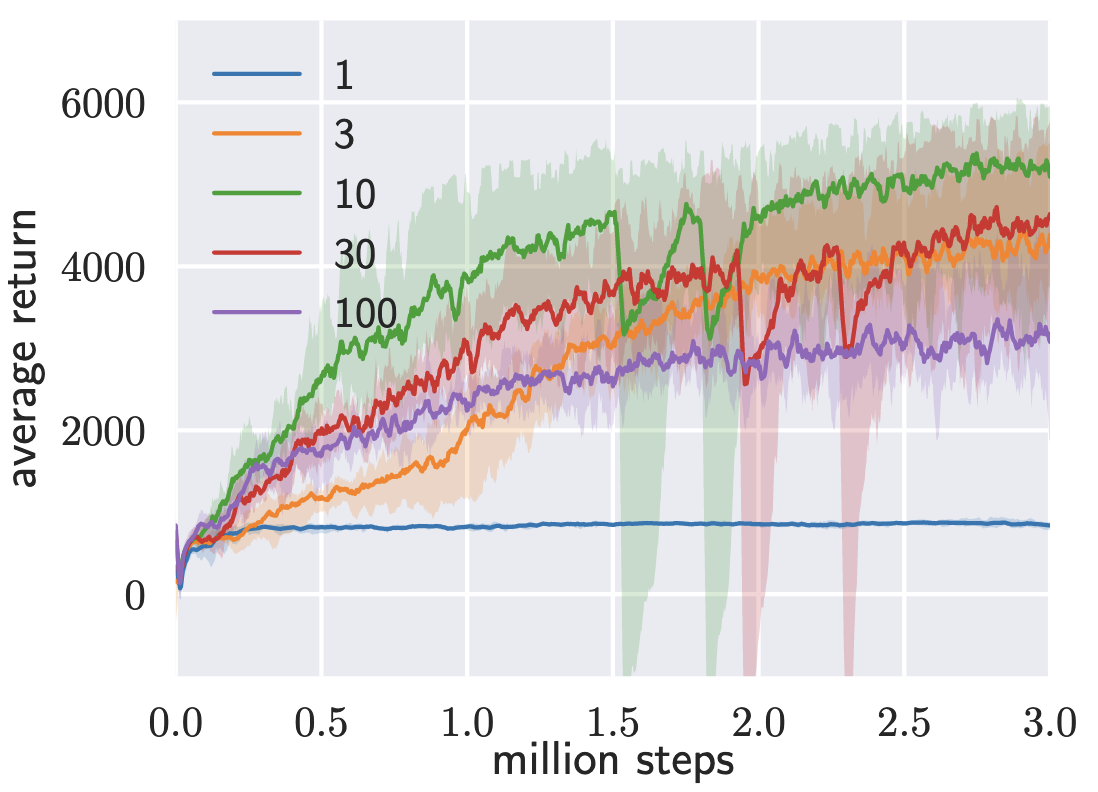
\includegraphics[width=0.4\textwidth]{fig3.png}
    \end{figure}

    Recall: original objective funciton augmented with maximum entropy is 
    \(
        \pi_{\text{MaxEnt}}^\ast = \arg \max_{\pi} \sum_{t=0}^T \mathbb{E}_{(s_t, a_t) \sim \rho_\pi}[r(s_t, a_t) + \alpha \mathcal{H}(\pi(\cdot \mid s_t))]
    \)

    In SAC algorithm, $\alpha=1$. So reward scaling plays a role that tunes the temperature

    \begin{itemize}
        \item For small reward magnitudes, the policy becomes nearly uniform, and consequently fails to exploit the reward signal, resulting in substantial degradation of performance. 
        \item For large reward magnitudes, the model learns quickly at first, but the policy then becomes nearly deterministic, leading to poor local minima due to lack of adequate exploration.
        \item With the right reward scaling, the model balances exploration and exploitation, leading to faster learning and better asymptotic performance
        \item The optimal reward scale varies between environments, and should be tuned for each task separately, remained as hyperparameter.
    \end{itemize}
\end{frame}

\begin{frame}{Experiments: compare with other algorithms}
    \begin{figure}
        \centering
        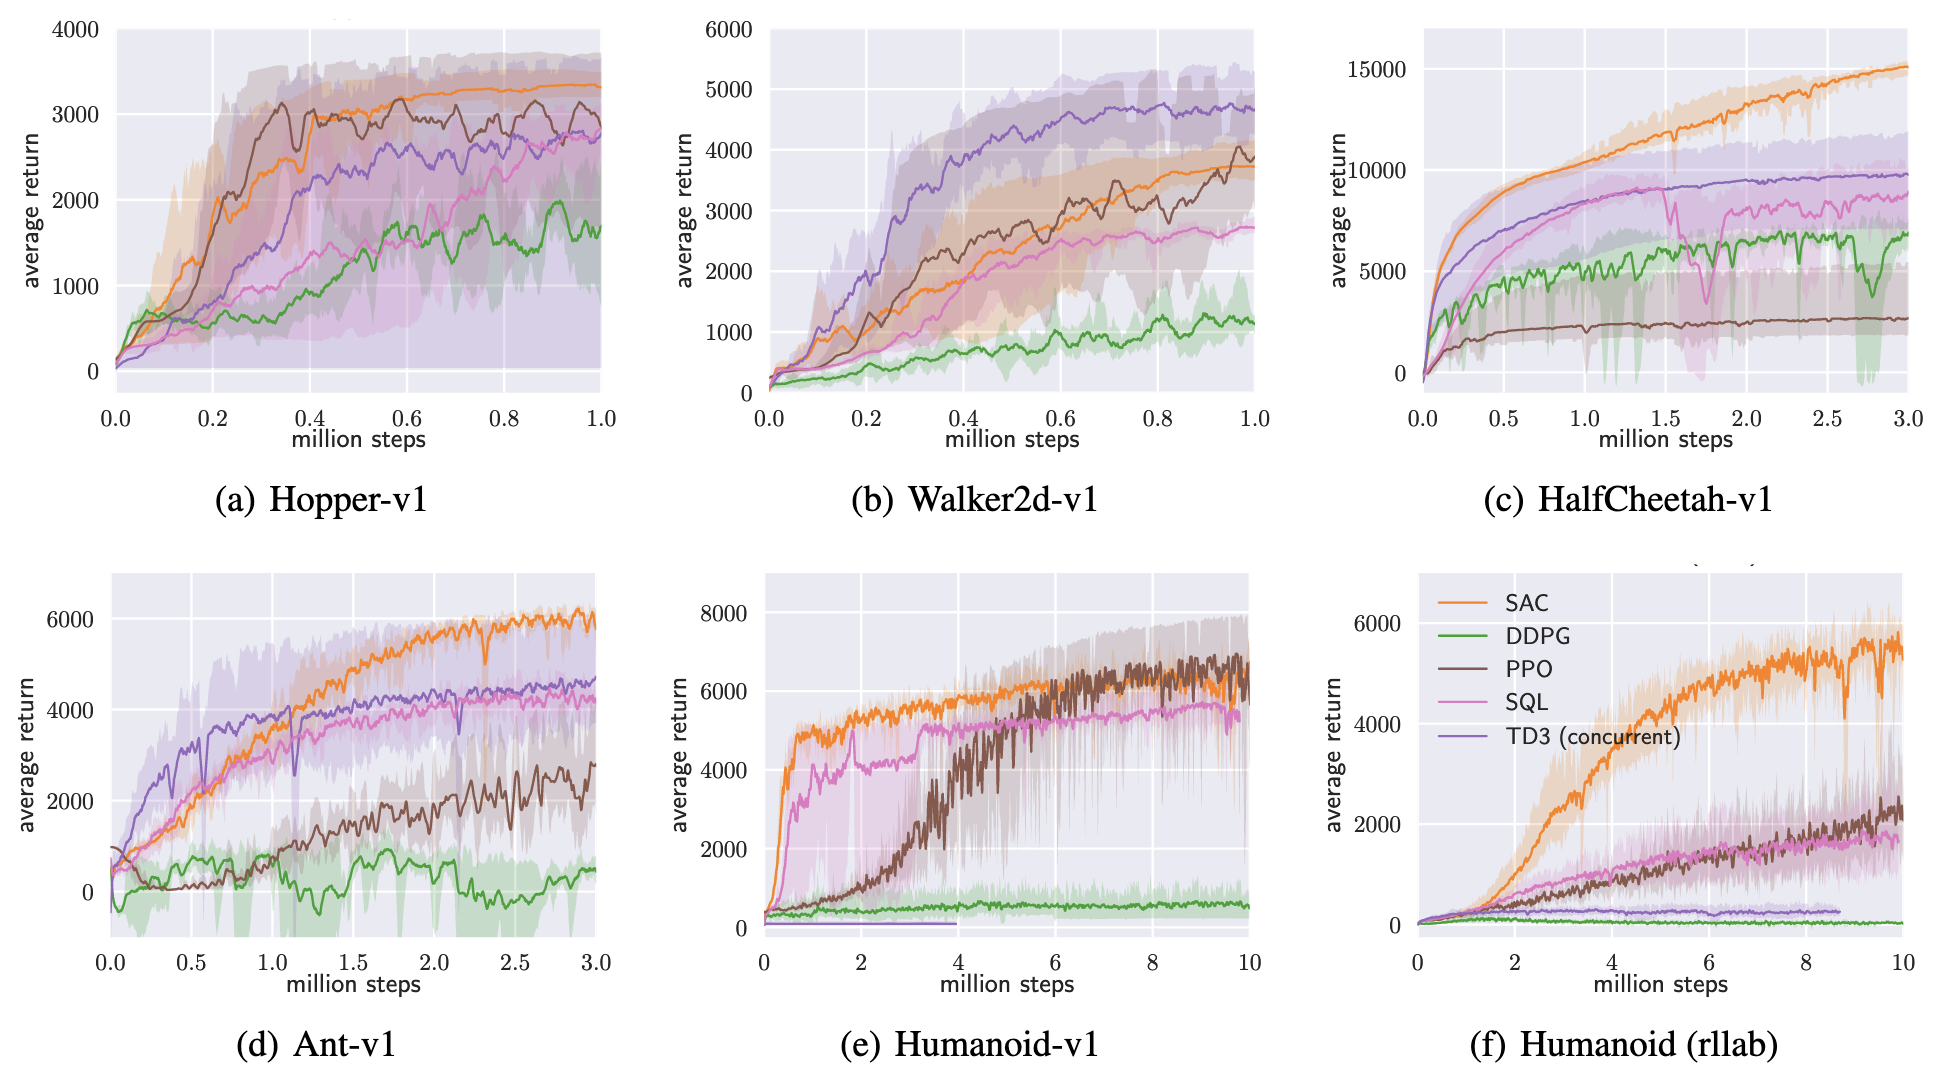
\includegraphics[width=0.6\textwidth]{fig1.png}
    \end{figure}


Compared SAC with DDPG, PPO, SQL, and TD3.
\begin{itemize}
    \item Figure shows the total average return of evaluation rollouts during training for DDPG, PPO and TD3
    \item turned off the exploration noise of DDPG and PPO
    \item evaluate for each 1000 step and mean result of 5 different random seeds
\end{itemize}
\end{frame}

\begin{frame}{Experiments: stochastic policy}
\begin{figure}
\centering

\includegraphics[width=0.4\textwidth]{fig2.png}
\end{figure}
Above figure shows comparison of SAC with stochastic policy and SAC with deterministic policy
Deterministic variant of SAC
\begin{itemize}
    \item those not maximize entropy
    \item closely resembles DDPG, with the exception of having two Q-functions
    \item hard target update
    \item using fixed rather than learned exploration noise
\end{itemize}

Above figure visualizes each five individual runs with both variants, initialized with different random seeds
\begin{itemize}
    \item It seems that entropy maximization can drastically stabilize training

\end{itemize}
\end{frame} 

\begin{frame}{End}
    Thank you
\end{frame}
\end{document}